%
%	Configure LaTeX to produce a PDF "book" using the memoir class
%

\documentclass[10pt,oneside]{memoir}

%
%	Generic Configuration for memoir-based documents
%

\usepackage{layouts}[2001/04/29]


% In case we need a glossary, or index
\usepackage{glossaries}
\glstoctrue
\makeglossaries
\makeindex


% Basic page layout configuration
\def\mychapterstyle{default}
\def\mypagestyle{headings}


% Use 8.5 x 11 inch page layout
%
%	8.5 x 11 layout for memoir-based documents
%


%%% need more space for ToC page numbers
\setpnumwidth{2.55em}
\setrmarg{3.55em}

%%% need more space for ToC section numbers
\cftsetindents{part}{0em}{3em}
\cftsetindents{chapter}{0em}{3em}
\cftsetindents{section}{3em}{3em}
\cftsetindents{subsection}{4.5em}{3.9em}
\cftsetindents{subsubsection}{8.4em}{4.8em}
\cftsetindents{paragraph}{10.7em}{5.7em}
\cftsetindents{subparagraph}{12.7em}{6.7em}

%%% need more space for LoF numbers
\cftsetindents{figure}{0em}{3.0em}

%%% and do the same for the LoT
\cftsetindents{table}{0em}{3.0em}

%%% set up the page layout
\settrimmedsize{\stockheight}{\stockwidth}{*}	% Use entire page
\settrims{0pt}{0pt}

\setlrmarginsandblock{1.5in}{1.5in}{*}
\setulmarginsandblock{1.5in}{1.5in}{*}

\setmarginnotes{17pt}{51pt}{\onelineskip}
\setheadfoot{\onelineskip}{2\onelineskip}
\setheaderspaces{*}{2\onelineskip}{*}
\checkandfixthelayout


% Use default packages for memoir setup
%
%	Default packages for memoir documents created by MultiMarkdown
%

\usepackage{fancyvrb}			% Allow \verbatim et al. in footnotes
\usepackage{graphicx}			% To enable including graphics in pdf's
\usepackage{booktabs}			% Better tables
\usepackage{tabulary}			% Support longer table cells
\usepackage[utf8]{inputenc}		% For UTF-8 support
\usepackage[T1]{fontenc}		% Use T1 font encoding for accented characters
\usepackage{xcolor}				% Allow for color (annotations)
\usepackage[sort&compress]{natbib} % Better bibliography support

\VerbatimFootnotes



% Configure default metadata to avoid errors
%
%	Configure default metadata in case it's missing to avoid errors
%

\def\myauthor{Author}
\def\defaultemail{}
\def\defaultposition{}
\def\defaultdepartment{}
\def\defaultaddress{}
\def\defaultphone{}
\def\defaultfax{}
\def\defaultweb{}


\def\mytitle{Title}
\def\subtitle{}
\def\keywords{}


\def\bibliostyle{plain}
% \def\bibliocommand{}

\def\myrecipient{}

% Overwrite with your own if desired
%\input{ftp-metadata}






\def\mytitle{ThesisDocumentsMelodyMatcher}
\def\myauthor{Jenee Hughes}
\def\latexmode{memoir}
%
%	Get ready for the actual document
%

\usepackage[
	plainpages=false,
	pdfpagelabels,
	pdftitle={\mytitle},
	pagebackref,
	pdfauthor={\myauthor},
	pdfkeywords={\keywords}
	]{hyperref}
\usepackage{memhfixc}


%
%	Configure information from metadata for use in title
%

\ifx\latexauthor\undefined
\else
	\def\myauthor{\latexauthor}
\fi

\ifx\subtitle\undefined
\else
	\addtodef{\mytitle}{}{ \\ \subtitle}
\fi

\ifx\affiliation\undefined
\else
	\addtodef{\myauthor}{}{ \\ \affiliation}
\fi

\ifx\address\undefined
\else
	\addtodef{\myauthor}{}{ \\ \address}
\fi

\ifx\phone\undefined
\else
	\addtodef{\myauthor}{}{ \\ \phone}
\fi

\ifx\email\undefined
\else
	\addtodef{\myauthor}{}{ \\ \email}
\fi

\ifx\event\undefined
\else
	\date[\mydate]{\today}
\fi
\title{\mytitle}
\author{\myauthor}

\ifx\mydate\undefined
\else
	\date{\mydate}
\fi


\ifx\theme\undefined
\else
	\usetheme{\theme}
\fi

\begin{document}


\chapterstyle{\mychapterstyle}
\pagestyle{\mypagestyle}

% Frontmatter
\frontmatter

% Title Page
\maketitle
\clearpage

%
% Copyright Page
%

\vspace*{\fill}
\setlength{\parindent}{0pt}

\ifx\mycopyright\undefined
\else
	\textcopyright{} \mycopyright
\fi

\begin{center}
	\framebox{ \parbox[t]{1.5in}{\centering Formatted for \LaTeX \\ 
	by MultiMarkdown}}
\end{center}

\setlength{\parindent}{1em}
\clearpage

\tableofcontents
%\listoffigures
%\listoftables


\mainmatter


The word corpus is Latin, and means ``body''[1].  In general, it's helpful to think of a text corpus as a ``body of text'' with some special constraints.

In linguistics, the term ``corpora'' refers to samples from various textual sources.
  
A ``text corpus''  refers to a large, structured body of text, consisting of those corpora (a.k.a. samples from various textual sources). 

In order for a text corpus to be useful, it must be a representative subset of the larger language it wishes to represent. 

If I'm trying to put together a general text corpus for the English language, then I should pull from many sources: books, newspapers, movie scripts, magazines, academic literature, etc. 

If one genre is over-represented in my corpora (text samples), then the resultant text corpus can be biased, and not useful for general purposes. For example: if I pull my all my corpora (text samples) from Wikipedia, my resulting text corpus is  likely to underrepresent most first-person and second-person nouns and verbs, since those are verboten in Wikipedia articles.
Uses of Text Corpora
A text corpus is generally used as the ``control'' set for comparing to data from linguistic experiments. 

Given a good text corpus, word frequency can be generated simply by counting the number of occurrences of every word that appears in the corpus. This frequency data can be used by other applications, like my Melody Matcher, to weight the possibility of resolving homophones[4], by calculating which words have a higher frequency count in the corpus. The higher the frequency, the are more common a word is, and the more likely it is to be heard.

In addition, given a text corpus, one can generate a dictionary of all words in the corpus. This dictionary can then be annotated with data such as part of speech, unique identifiers for homographs[2], and phonetic spelling. 

The word frequencies in the UNISYN dictionary were generated by scrapping several text corpuses for their frequency data: pre-calculated frequencies from the British National Corpus and Maptask, plus some frequencies derived from Time articles and online texts such as Gutenberg.
To review:
A text corpus is a large, structured set of texts, used to do comparative analysis on linguistic data sets.

Isn't it exciting to learn new things?

Footnotes for Semi-Relevant Tangents
[1] Fun fact! It's the same corpus that we use in habeas corpus (a Latin phrase that is directly translated to ``You have the body'', and refers to the legal mechanism in which a suspect cannot be held indefinitely without trial).

[2] Homographs are orthographic words that are spelled identically. Typically, homographs are also pronounced differently, which makes them homographic heterophones. For example, there are two different pronunciations of ``does'' : the ``multiple female deer'' does (doze), and the ``third-person singular present indicative form of `do''' does (duhz). If the words are spelled identically AND pronounced identically, then then are homographic[2] homophones[4], which are commonly known as homonyms[5].

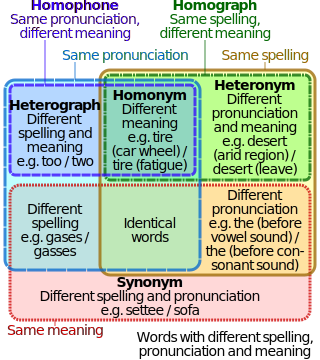
\includegraphics[keepaspectratio,width=\textwidth,height=0.75\textheight]{Homograph_homophone_venn_diagram.tiff}

(Image Source: Wikimedia commons)

[3] Heterographs are orthographic words that are spelled differently. Typically, words are only called heterographs if they are also pronounced differently, making them heterographic homophones[4]. The word does is a heterographic homophone with two different pronunciations: the ``multiple female deer'' does (doze), and the ``third-person singular present indicative form of `do''' does (duhz).   (Most words in the English language are heterographic heterophones; that is, spelled and pronounced uniquely. Because this is the default state of a word set, we rarely describe them in terms of homo\slash hetero phones\slash graphs.  As such, the only time a word set is likely to be described as heterographic is if it is a homophone. 

[4] Homophones are orthographic words that are pronounced identically, but typically spelled differently. For example, the banes of every spelling Nazi, there, their, and they're, are heterographic[3] homophones. Alternatively, to, too, and two are also heterographic homophones.  If a homophone set is also homographic (that is, spelled identically as well as pronounced identically), then we refer to them as homonyms. As such, the only time the words in a set are likely to be labelled ``homophones'' is if they are also heterographic.

[5] Homonyms are orthographic words that are pronounced and spelled identically, but defined differently. For example, depending on context, the word ``left'' can mean left (the opposite of right), or left (the past tense of leave). Homonyms can also be referred to as homographic[2] homophones[4]. See Wikipedia if you don't believe me!

%
%	MultiMarkdown default footer file
%


% Back Matter
\if@mainmatter
	we're in main
	\backmatter
\fi


% Bibliography

\ifx\bibliocommand\undefined
\else
	\bibliographystyle{\bibliostyle}
	\bibliocommand
\fi



% Glossary
\printglossaries


% Index
\printindex



\end{document}
